\usetikzlibrary{arrows.meta, calc, fit, matrix, patterns, shapes.misc}

\providecommand{\computer}{%
    
\includegraphics[width=1cm]{../common/Noun_project_216.pdf}
}
\providecommand{\switch}{%
    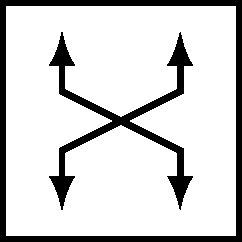
\includegraphics[width=0.9cm]{../common/fig-switch.pdf}
}
\providecommand{\bigswitch}{%
    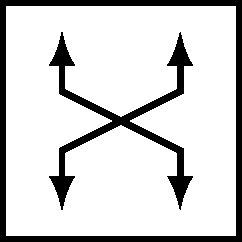
\includegraphics[width=1.4cm]{../common/fig-switch.pdf}
}
\providecommand{\router}{%
    
\includegraphics[width=0.9cm]{../common/fig-router.pdf}
}


\begin{frame}{sequence number wraparound}
    \begin{itemize}
    \item protocol so far requires arbitrarily large sequence numbers
        \begin{itemize}
        \item doing $<$ and $>$ checks on sequence number, so they need to increase
        \end{itemize}
    \item would like to use smaller sequence numbers
        \begin{itemize}
        \item think: transferring multi-gigabyte file
        \end{itemize}
    \item question: what goes wrong when we reuse sequeunce numbers?
    \end{itemize}
\end{frame}

\begin{frame}{sender/receiver desync: missing ACKs}
\begin{tikzpicture}
\tikzset{
    seqlist/.style={tight matrix,nodes={text width=.8cm,minimum height=.8cm},column sep=.6mm},
    dots/.style={draw=none,execute at begin node=\ldots,anchor=center,font=\huge,text width=1cm,align=center},
    region mark/.style={very thick,decorate,decoration={brace,mirror}},
    region mark label/.style={midway,below,align=center},
    verified/.style={pattern color=black!30,pattern=checkerboard},
    ack sent not recvd/.style={fill=blue!60},
    unsent ready/.style={pattern color=yellow!30!black,pattern=checkerboard},
    unsent/.style={pattern=crosshatch dots,pattern color=violet!70},
}
\begin{scope}[name prefix=s-]
    \matrix[seqlist] (window) {
        |[dots,alias=window-start]| ~ \& |[alias=after-window-start,verified,alias=LAR]| ~ \&
        |[ack sent not recvd,alias=after LAR]| ~ \& |[ack sent not recvd]| ~ \& |[ack sent not recvd]| ~ \& 
        |[ack sent not recvd,alias=LFS]| ~ \& 
        |[alias=after LFS,unsent]| ~ \& |[unsent,alias=before-window-end]| ~  \&
        |[unsent]| ~  \&
        |[unsent]| ~  \&
        |[unsent]| ~  \&
        |[unsent,alias=before-window-end]| ~  \&
        \& |[alias=window-end,dots]| \\
    };
    \node[anchor=east] at (window-start.west) {sender};
    \draw[thick,Latex-] (LAR.north) -- ++(0,.5) node[above,align=center] (LAR label) {(LAR)\\last ACK recv'd};
    \draw[thick,Latex-] (LFS.north) -- ++(0,.5) node[above,align=center] (LFS label) {(LFS)\\last frame sent};
\end{scope}
\begin{scope}[name prefix=r-,yshift=-3cm]
    \matrix[seqlist] (window) {
        |[dots,alias=window-start]| ~ \& |[alias=after-window-start,verified]| ~ \& 
        |[alias=after LAR,ack sent not recvd]| ~ \& |[ack sent not recvd]| ~ \& 
        |[ack sent not recvd]| ~ \& |[alias=LFR,ack sent not recvd]| ~ \&
        |[unsent ready,alias=after LFR]| ~ \& |[unsent ready,alias=after after LFR]| ~ \&
        |[unsent ready]| ~ \& |[unsent ready,alias=LAF]| ~ \& 
        |[alias=after LAF,unsent]| ~ \& |[unsent,alias=before-window-end]| ~ \& |[alias=window-end,dots]| \\
    };
    \node[anchor=east] at (window-start.west) {receiver};
    \draw[thick,Latex-] (LFR.north) -- ++(0,.5) node[above,align=center] {(LFR)\\last frame recv'd*};
    \draw[thick,Latex-] (LAF.north) -- ++(0,.5) node[above,align=center] {(LAF)\\last accepted frame};
    \draw[region mark] ([yshift=-.1cm]after LAR.south west) -- ([yshift=-.1cm]LFR.south east)
        node[region mark label] {resent if \\ ACK lost};
    \draw[region mark] ([yshift=-.1cm]after LFR.south west) -- ([yshift=-.1cm]LAF.south east)
        node[region mark label] {expected if \\ ACK not lost};
\end{scope}
\begin{visibleenv}<2->
\node[draw=red,ultra thick,fit=(s-after LAR) (r-LAF),label={[red,align=left,fill=white,fill opacity=0.95]west:need unique \\ numbers for all these}] {};
\end{visibleenv}
\begin{visibleenv}<3->
\foreach \x/\lbl in {2/4,3/5,4/6,5/7,6/0,7/1,8/2,9/3,10/4,11/5,12/6,13/7} {
    \node[fill=white,font=\small,text=red,circle,draw=red,ultra thick,anchor=south west,inner sep=0.1mm] at ([xshift=\x * .935cm - 0.4cm]s-window-start.north west) {\lbl};
}
\end{visibleenv}
\end{tikzpicture}
\end{frame}

\begin{frame}{wraparound}
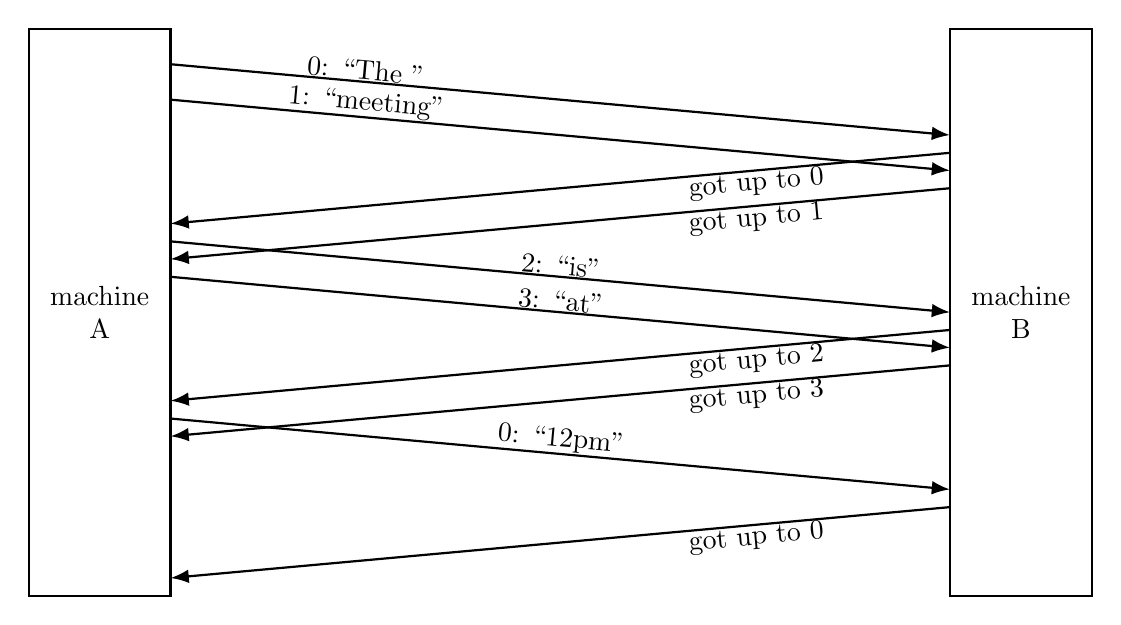
\begin{tikzpicture}
\tikzset{
    box/.style={thick},
    message/.style={draw,thick,-Latex},
    failure/.style={draw,ultra thick,red,cross out,minimum width=1cm,minimum height=1cm},
    every node/.style={inner sep=0.1mm},
}
\begin{scope}[xshift=1cm,x=0.9cm,y=0.9cm]
\draw[box] (0, 0) rectangle ++(2, -8) 
    node[midway,align=center] {machine\\A};
\draw[box] (13, 0) rectangle ++(2, -8) 
    node[midway,align=center] {machine\\B};
\draw[message] (2, -0.5) -- (13, -1.5) node[pos=0.25,above,sloped] {\myemph{0}: ``The ''};
\draw[message] (13, -1.75) -- (2, -2.75) node[pos=0.25,sloped,below] {got up to \myemph{0}};
\draw[message] (2, -1) -- (13, -2) node[pos=0.25, above, sloped] {\myemph{1}: ``meeting''};
\draw[message] (13, -2.25) -- (2, -3.25) node[pos=0.25, sloped,below] {got up to \myemph{1}};

% in response to got 0
\draw[message] (2, -3) -- (13, -4) node[pos=0.5, above, sloped] {\myemph{2}: ``is''};
\draw[message] (13, -4.25) -- (2, -5.25) node[pos=0.25, sloped,below] {got up to \myemph{2}};
% in response to got 1
\draw[message] (2, -3.5) -- (13, -4.5) node[pos=0.5, above, sloped] {\myemph{3}: ``at''};
\draw[message] (13, -4.75) -- (2, -5.75) node[pos=0.25, sloped,below] {got up to \myemph{3}};

% in response to got 2
\draw[message] (2, -5.5) -- (13, -6.5) node[pos=0.5, above, sloped] {\myemph{0}: ``12pm''};
\draw[message] (13, -6.75) -- (2, -7.75) node[pos=0.25, sloped,below] {got up to \myemph{0}};
\end{scope}
\end{tikzpicture}
\end{frame}

\begin{frame}{loss and resend?}
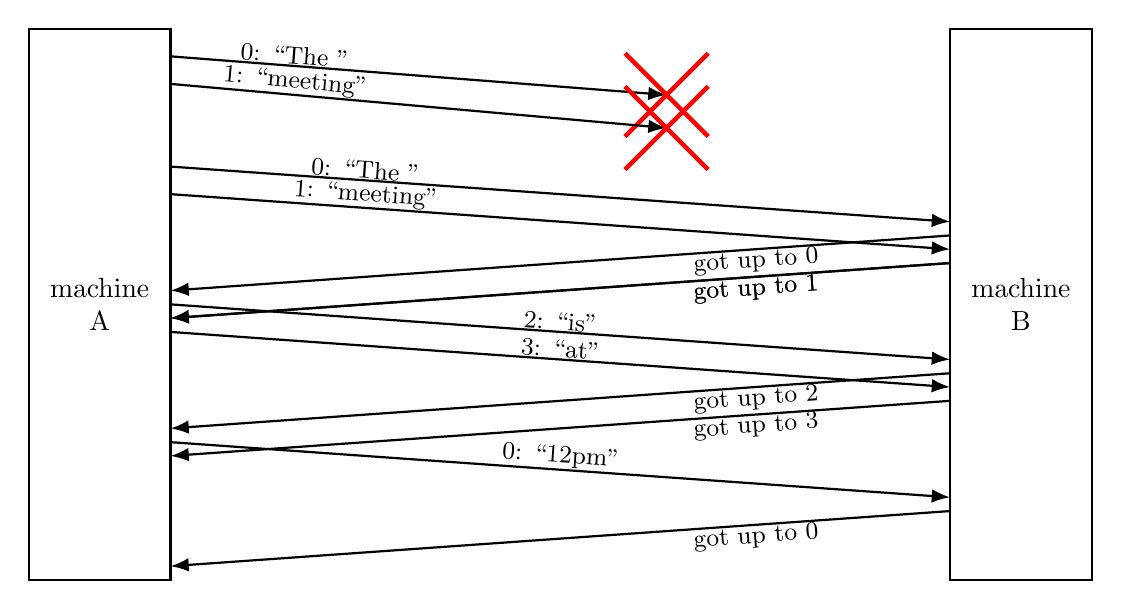
\begin{tikzpicture}
\tikzset{
    box/.style={thick},
    message/.style={draw,thick,-Latex,font=\small},
    failure/.style={draw,ultra thick,red,cross out,minimum width=1cm,minimum height=1cm},
    every node/.style={inner sep=0.1mm},
}
\begin{scope}[xshift=1cm,x=0.9cm,y=0.7cm]
\draw[box] (0, 2) rectangle ++(2, -10) 
    node[midway,align=center] {machine\\A};
\draw[box] (13, 2) rectangle ++(2, -10) 
    node[midway,align=center] {machine\\B};
\draw[message] (2, 2-0.5) -- (9, 2-1.2) node[pos=0.25,above,sloped] {\myemph{0}: ``The ''} node[failure] {};
\draw[message] (2, 2-1) -- (9, 2-1.8) node[pos=0.25, above, sloped] {\myemph{1}: ``meeting''} node[failure] {};
\draw[message] (13, -2.25) -- (2, -3.25) node[pos=0.25, sloped,below] {got up to \myemph{1}};
\draw[message] (2, -0.5) -- (13, -1.5) node[pos=0.25,above,sloped] {\myemph{0}: ``The ''};
\draw[message] (13, -1.75) -- (2, -2.75) node[pos=0.25,sloped,below] {got up to \myemph{0}};
\draw[message] (2, -1) -- (13, -2) node[pos=0.25, above, sloped] {\myemph{1}: ``meeting''};
\draw[message] (13, -2.25) -- (2, -3.25) node[pos=0.25, sloped,below] {got up to \myemph{1}};

% in response to got 0
\draw[message] (2, -3) -- (13, -4) node[pos=0.5, above, sloped] {\myemph{2}: ``is''};
\draw[message] (13, -4.25) -- (2, -5.25) node[pos=0.25, sloped,below] {got up to \myemph{2}};
% in response to got 1
\draw[message] (2, -3.5) -- (13, -4.5) node[pos=0.5, above, sloped] {\myemph{3}: ``at''};
\draw[message] (13, -4.75) -- (2, -5.75) node[pos=0.25, sloped,below] {got up to \myemph{3}};

% in response to got 2
\draw[message] (2, -5.5) -- (13, -6.5) node[pos=0.5, above, sloped] {\myemph{0}: ``12pm''};
\draw[message] (13, -6.75) -- (2, -7.75) node[pos=0.25, sloped,below] {got up to \myemph{0}};
\end{scope}
\end{tikzpicture}
\end{frame}

\begin{frame}{very bad reordering}
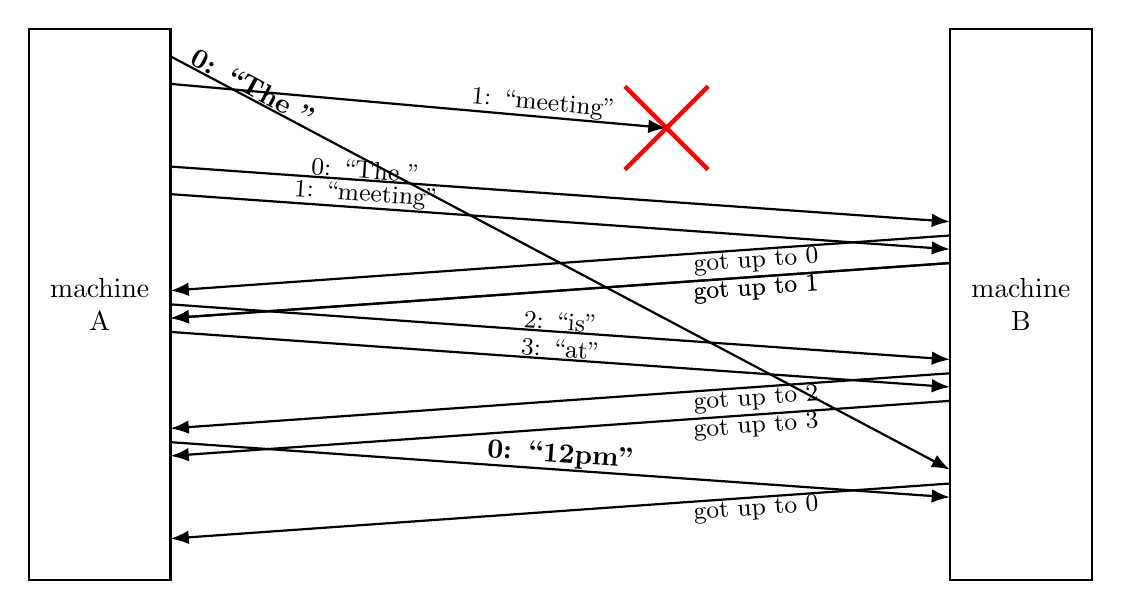
\begin{tikzpicture}
\tikzset{
    box/.style={thick},
    message/.style={draw,thick,-Latex,font=\small},
    failure/.style={draw,ultra thick,red,cross out,minimum width=1cm,minimum height=1cm},
    every node/.style={inner sep=0.1mm},
}
\begin{scope}[xshift=1cm,x=0.9cm,y=0.7cm]
\draw[box] (0, 2) rectangle ++(2, -10) 
    node[midway,align=center] {machine\\A};
\draw[box] (13, 2) rectangle ++(2, -10) 
    node[midway,align=center] {machine\\B};
\draw[message] (2, 2-0.5) -- (13, -6) node[pos=0.1,above,sloped,font=\bfseries] {\myemph{0}: ``The ''};
\draw[message] (2, 2-1) -- (9, 2-1.8) node[pos=0.75, above, sloped] {\myemph{1}: ``meeting''} node[failure] {};
\draw[message] (13, -2.25) -- (2, -3.25) node[pos=0.25, sloped,below] {got up to \myemph{1}};
\draw[message] (2, -0.5) -- (13, -1.5) node[pos=0.25,above,sloped] {\myemph{0}: ``The ''};
\draw[message] (13, -1.75) -- (2, -2.75) node[pos=0.25,sloped,below] {got up to \myemph{0}};
\draw[message] (2, -1) -- (13, -2) node[pos=0.25, above, sloped] {\myemph{1}: ``meeting''};
\draw[message] (13, -2.25) -- (2, -3.25) node[pos=0.25, sloped,below] {got up to \myemph{1}};

% in response to got 0
\draw[message] (2, -3) -- (13, -4) node[pos=0.5, above, sloped] {\myemph{2}: ``is''};
\draw[message] (13, -4.25) -- (2, -5.25) node[pos=0.25, sloped,below] {got up to \myemph{2}};
% in response to got 1
\draw[message] (2, -3.5) -- (13, -4.5) node[pos=0.5, above, sloped] {\myemph{3}: ``at''};
\draw[message] (13, -4.75) -- (2, -5.75) node[pos=0.25, sloped,below] {got up to \myemph{3}};

% in response to got 2
\draw[message] (2, -5.5) -- (13, -6.5) node[pos=0.5, above, sloped,font=\bfseries] {\myemph{0}: ``12pm''};
% in response to BOGUS got 0
\draw[message] (13, -6.25) -- (2, -7.25) node[pos=0.25, sloped,below] {got up to \myemph{0}};
\end{scope}
\end{tikzpicture}
\end{frame}

% FIXME: show link getting dis/reconnected
\begin{frame}{possible reason}
\begin{tikzpicture}
\tikzset{
    connect one/.style={draw,very thick,Latex-Latex},
    computer/.style={inner sep=0mm,outer sep=0mm,execute at begin node={\computer}},
    switch/.style={inner sep=0mm,outer sep=0mm,execute at begin node={\switch}},
    router/.style={inner sep=0mm,outer sep=0mm,execute at begin node={\router}},
    big switch/.style={inner sep=0mm,outer sep=0mm,execute at begin node={\bigswitch}},
    packet/.style={minimum width=.4cm,minimum height=0.2cm,inner sep=0mm,outer sep=0mm,draw},
    packet lg/.style={minimum width=.6cm,minimum height=0.2cm,inner sep=0mm,outer sep=0mm,draw},
}
\node[computer] (start) at (0,0) {};
\node[computer] (end)  at (13,0) {};
\node[router] (pre1) at (3, 3) {};
\node[router] (pre2) at (4, .5) {};
\node[router] (pre3) at (5, 3) {};
\node[router] (A) at (6, 1) {};
\node[router] (B) at (7, -1) {};
\node[router] (C) at (8, 3) {};
\node[router] (D) at (11, 0) {};
\
\node[router] (E) at (7.5, -2) {};
\foreach \x/\y in {start/pre1,pre1/pre2,pre2/pre3,pre3/A,A/B,B/C,C/D,D/end,start/E,E/end} {
    \draw[connect one] (\x) -- (\y);
}
\node[font=\small,draw,fill=white] at ($(C)!0.5!(D)$) {\myemph{0}: ``The ''};
\node[font=\small,draw,fill=white] at ($(E)!0.7!(start)$) {\myemph{0}: ``12pm''};
\end{tikzpicture}
\end{frame}

\begin{frame}{sequence numbers in practice}
    \begin{itemize}
    \item TCP tries to assume 120 second ``maximum segment lifetime''
        \begin{itemize}
        \item segment = TCP's name for a packet
        \end{itemize}
    \item original TCP used 32-bit sequence number identifying \textit{byte} number (not segment number)
    \item problem: means wraparound happens on modern (Gigibit+) links in seconds!
    \vspace{.5cm}
    \item<2-> workaround: add \textit{additional} 32-bit timestamp field
        \begin{itemize}
        \item used to detect/discard duplicates
        \item can also be used to set timeouts and/or window sizes
        \end{itemize}
    \end{itemize}
\end{frame}
